% Options for packages loaded elsewhere
\PassOptionsToPackage{unicode}{hyperref}
\PassOptionsToPackage{hyphens}{url}
%
\documentclass[
  12pt,
]{article}
\usepackage{lmodern}
\usepackage{amssymb,amsmath}
\usepackage{ifxetex,ifluatex}
\ifnum 0\ifxetex 1\fi\ifluatex 1\fi=0 % if pdftex
  \usepackage[T1]{fontenc}
  \usepackage[utf8]{inputenc}
  \usepackage{textcomp} % provide euro and other symbols
\else % if luatex or xetex
  \usepackage{unicode-math}
  \defaultfontfeatures{Scale=MatchLowercase}
  \defaultfontfeatures[\rmfamily]{Ligatures=TeX,Scale=1}
\fi
% Use upquote if available, for straight quotes in verbatim environments
\IfFileExists{upquote.sty}{\usepackage{upquote}}{}
\IfFileExists{microtype.sty}{% use microtype if available
  \usepackage[]{microtype}
  \UseMicrotypeSet[protrusion]{basicmath} % disable protrusion for tt fonts
}{}
\makeatletter
\@ifundefined{KOMAClassName}{% if non-KOMA class
  \IfFileExists{parskip.sty}{%
    \usepackage{parskip}
  }{% else
    \setlength{\parindent}{0pt}
    \setlength{\parskip}{6pt plus 2pt minus 1pt}}
}{% if KOMA class
  \KOMAoptions{parskip=half}}
\makeatother
\usepackage{xcolor}
\IfFileExists{xurl.sty}{\usepackage{xurl}}{} % add URL line breaks if available
\IfFileExists{bookmark.sty}{\usepackage{bookmark}}{\usepackage{hyperref}}
\hypersetup{
  pdftitle={Officials in NBA Games with Prolific Player Scoring},
  hidelinks,
  pdfcreator={LaTeX via pandoc}}
\urlstyle{same} % disable monospaced font for URLs
\usepackage[left=12mm, right=12mm, top=15mm, bottom=15mm]{geometry}
\usepackage{graphicx,grffile}
\makeatletter
\def\maxwidth{\ifdim\Gin@nat@width>\linewidth\linewidth\else\Gin@nat@width\fi}
\def\maxheight{\ifdim\Gin@nat@height>\textheight\textheight\else\Gin@nat@height\fi}
\makeatother
% Scale images if necessary, so that they will not overflow the page
% margins by default, and it is still possible to overwrite the defaults
% using explicit options in \includegraphics[width, height, ...]{}
\setkeys{Gin}{width=\maxwidth,height=\maxheight,keepaspectratio}
% Set default figure placement to htbp
\makeatletter
\def\fps@figure{htbp}
\makeatother
\setlength{\emergencystretch}{3em} % prevent overfull lines
\providecommand{\tightlist}{%
  \setlength{\itemsep}{0pt}\setlength{\parskip}{0pt}}
\setcounter{secnumdepth}{-\maxdimen} % remove section numbering
\usepackage{fontspec} \usepackage{background} \usepackage{float} \backgroundsetup{ scale=1, color=black, opacity=0.20, angle=0, pages=all, contents={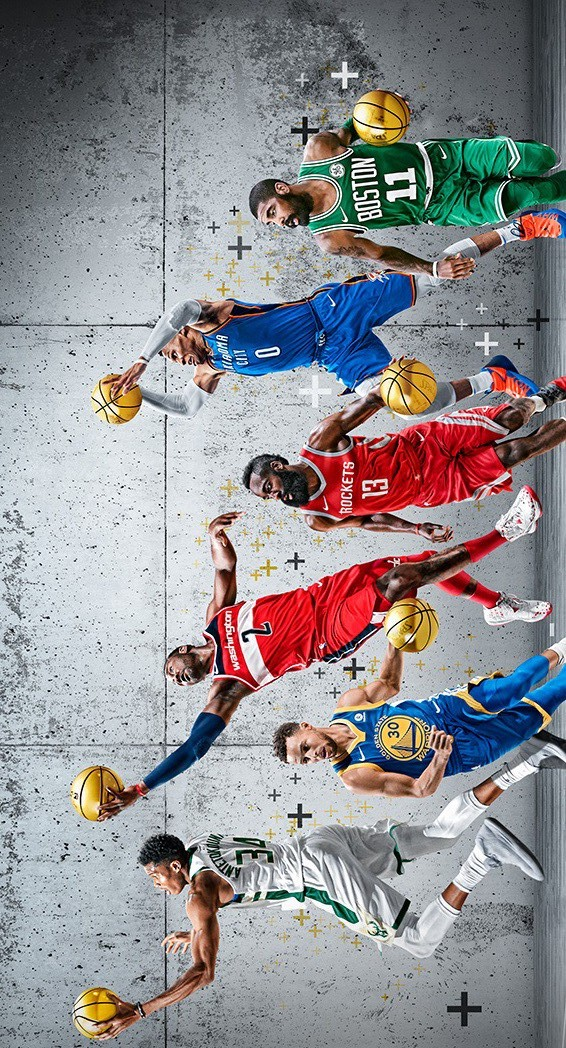
\includegraphics[width=25cm,height=40cm]{nba_action_02.jpg}} } \setmainfont{Avenir}
\usepackage{booktabs}
\usepackage{longtable}
\usepackage{array}
\usepackage{multirow}
\usepackage{wrapfig}
\usepackage{float}
\usepackage{colortbl}
\usepackage{pdflscape}
\usepackage{tabu}
\usepackage{threeparttable}
\usepackage{threeparttablex}
\usepackage[normalem]{ulem}
\usepackage{makecell}
\usepackage{xcolor}

\title{Officials in NBA Games with Prolific Player Scoring}
\author{}
\date{\vspace{-2.5em}}

\begin{document}
\maketitle

2021-04-21

Stats MAS405 Spring 2021

Dave Zes

\hypertarget{introduction}{%
\subsection{Introduction}\label{introduction}}

In the NBA, are some officials more likely than others to have
officiated a game with a prolific individual player performance?
Utilizing regular season NBA game and player data spanning 2004-11-02 to
2020-03-11, we produce frequencies of officials in games where a player
scored more than 55 points.

\hypertarget{results}{%
\subsection{Results}\label{results}}

Table 1 shows game information for all games in our data where a player
(name) scored more than 55 points.

\begin{table}[ht]
\scriptsize
\centering
\begin{tabular}{rllrlllrr}
  \hline
date & VT & HT & min & refs & team & name & min.1 & pts \\ 
  \hline
20050212 & ORL & PHI & 240 & Mike Callahan, James Capers Jr., Anthony Jordan & PHI & Allen Iverson &  42 &  60 \\ 
  20050320 & CLE & TOR & 240 & Michael Henderson, Jess Kersey, Jack Nies & CLE & LeBron James &  48 &  56 \\ 
  20051220 & DAL & LAL & 240 & Steve Javie, Olandis Poole, Leroy Richardson & LAL & Kobe Bryant &  32 &  62 \\ 
  20060122 & TOR & LAL & 240 & Kevin Fehr, Bill Kennedy, Bill Spooner & LAL & Kobe Bryant &  41 &  81 \\ 
  20061111 & UTZ & MIL & 240 & James Capers Jr., Olandis Poole, Greg Willard & MIL & Michael Redd &  45 &  57 \\ 
  20061217 & WAS & LAL & 265 & Dan Crawford, Courtney Kirkland, Jason Phillips & WAS & Gilbert Arenas &  49 &  60 \\ 
  20061229 & LAL & CHA & 315 & Sean Corbin, Leroy Richardson, Derrick Stafford & LAL & Kobe Bryant &  54 &  58 \\ 
  20070316 & POR & LAL & 265 & Sean Corbin, Joe DeRosa, Eli Roe & LAL & Kobe Bryant &  49 &  65 \\ 
  20070322 & LAL & MEM & 240 & James Capers Jr., Bob Delaney, Courtney Kirkland & LAL & Kobe Bryant &  45 &  60 \\ 
  20090202 & LAL & NYK & 240 & Mark Ayotte, Bob Delaney, David Jones & LAL & Kobe Bryant &  36 &  61 \\ 
  20120304 & BRK & CHA & 240 & Derrick Collins, Derek Richardson, Bill Spooner & BRK & Deron Williams &  37 &  57 \\ 
  20140124 & CHA & NYK & 240 & Curtis Blair, David Guthrie, Ken Mauer & NYK & Carmelo Anthony &  38 &  62 \\ 
  20140303 & CHA & MIA & 240 & Eric Lewis, Bennett Salvatore, Ben Taylor & MIA & LeBron James &  41 &  61 \\ 
  20150312 & CLE & SAS & 265 & Eric Lewis, Derrick Stafford, Dedric Taylor & CLE & Kyrie Irving &  46 &  57 \\ 
  20160125 & CHA & SAC & 290 & Steve Anderson, Kane Fitzgerald, Zach Zarba & SAC & DeMarcus Cousins &  45 &  56 \\ 
  20160221 & NOP & DET & 240 & Pat Fraher, Lauren Holtkamp-Sterling, Monty McCutchen & NOP & Anthony Davis &  43 &  59 \\ 
  20160413 & UTZ & LAL & 240 & David Guthrie, Monty McCutchen, Haywoode Workman & LAL & Kobe Bryant &  42 &  60 \\ 
  20161205 & IND & GSW & 240 & Brett Nansel, Kevin Scott, Sean Wright & GSW & Klay Thompson &  29 &  60 \\ 
  20170307 & POR & OKC & 240 & Bill Spooner, Justin Van Duyne, James Williams & OKC & Russell Westbrook &  35 &  58 \\ 
  20170324 & PHX & BOS & 240 & Matt Boland, Eric Dalen, Bill Kennedy & PHX & Devin Booker &  44 &  70 \\ 
  20170329 & OKC & ORL & 265 & Curtis Blair, Michael Smith, Derrick Stafford & OKC & Russell Westbrook &  41 &  57 \\ 
  20170408 & UTZ & POR & 240 & Ron Garretson, Justin Van Duyne, James Williams & POR & Damian Lillard &  41 &  59 \\ 
  20171103 & CLE & WAS & 240 & Nick Buchert, Bill Kennedy, Haywoode Workman & CLE & LeBron James &  42 &  57 \\ 
  20171105 & UTZ & HOU & 240 & Eric Lewis, Ben Taylor, Josh Tiven & HOU & James Harden &  35 &  56 \\ 
  20180130 & ORL & HOU & 240 & Bennie Adams, Tony Brown, Dedric Taylor & HOU & James Harden &  46 &  60 \\ 
  20180328 & ATL & MIN & 240 & Eric Lewis, J.T. Orr, Michael Smith & MIN & Karl-Anthony Towns &  41 &  56 \\ 
  20181117 & PHI & CHA & 265 & Brett Nansel, Michael Smith, Zach Zarba & CHA & Kemba Walker &  45 &  60 \\ 
  20190110 & OKC & SAS & 290 & Brent Barnaky, Jason Phillips, Dedric Taylor & SAS & LaMarcus Aldridge &  48 &  56 \\ 
  20190114 & MEM & HOU & 240 & Ed Malloy, Rodney Mott, Gediminas Petraitis & HOU & James Harden &  34 &  57 \\ 
  20190116 & BRK & HOU & 265 & Curtis Blair, Phenizee Ransom, Sean Wright & HOU & James Harden &  45 &  58 \\ 
  20190123 & HOU & NYK & 240 & Brent Barnaky, Pat Fraher, Natalie Sago & HOU & James Harden &  40 &  61 \\ 
  20190228 & MIA & HOU & 240 & Tony Brothers, Mitchell Ervin, Brian Forte & HOU & James Harden &  43 &  58 \\ 
  20190320 & HOU & MEM & 265 & Marat Kogut, Jason Phillips, Derek Richardson & HOU & James Harden &  45 &  57 \\ 
  20190322 & SAS & HOU & 240 & Tony Brown, Aaron Smith, Zach Zarba & HOU & James Harden &  36 &  61 \\ 
  20190325 & PHX & UTZ & 240 & Derrick Collins, Kane Fitzgerald, Justin Van Duyne & PHX & Devin Booker &  41 &  59 \\ 
  20191030 & HOU & WAS & 240 & James Capers Jr., Jason Goldenberg, Kevin Scott & HOU & James Harden &  37 &  59 \\ 
  20191108 & BRK & POR & 240 & Mitchell Ervin, Scott Twardoski, Zach Zarba & POR & Damian Lillard &  40 &  60 \\ 
  20191130 & ATL & HOU & 240 & John Goble, Karl Lane, Leroy Richardson & HOU & James Harden &  30 &  60 \\ 
  20200120 & GSW & POR & 265 & J.B. DeRosa, Kane Fitzgerald, Brian Forte & POR & Damian Lillard &  45 &  61 \\ 
   \hline
\end{tabular}
\caption{NBA games in data where player scored more than 55 points.} 
\label{tabbig}
\end{table}


\newpage

\begingroup\fontsize{7pt}{7pt}\selectfont
\begin{longtable}{lr}
  \hline
official & numGames \\ 
  \hline
Eric Lewis &   4 \\ 
  James Capers Jr. &   4 \\ 
  Zach Zarba &   4 \\ 
  Bill Kennedy &   3 \\ 
  Bill Spooner &   3 \\ 
  Curtis Blair &   3 \\ 
  Dedric Taylor &   3 \\ 
  Derrick Stafford &   3 \\ 
  Jason Phillips &   3 \\ 
  Justin Van Duyne &   3 \\ 
  Kane Fitzgerald &   3 \\ 
  Leroy Richardson &   3 \\ 
  Michael Smith &   3 \\ 
  Ben Taylor &   2 \\ 
  Bob Delaney &   2 \\ 
  Brent Barnaky &   2 \\ 
  Brett Nansel &   2 \\ 
  Brian Forte &   2 \\ 
  Courtney Kirkland &   2 \\ 
  David Guthrie &   2 \\ 
  Derek Richardson &   2 \\ 
  Derrick Collins &   2 \\ 
  Haywoode Workman &   2 \\ 
  James Williams &   2 \\ 
  Kevin Scott &   2 \\ 
  Mitchell Ervin &   2 \\ 
  Monty McCutchen &   2 \\ 
  Olandis Poole &   2 \\ 
  Pat Fraher &   2 \\ 
  Sean Corbin &   2 \\ 
  Sean Wright &   2 \\ 
  Tony Brown &   2 \\ 
  Aaron Smith &   1 \\ 
  Anthony Jordan &   1 \\ 
  Bennett Salvatore &   1 \\ 
  Bennie Adams &   1 \\ 
  Dan Crawford &   1 \\ 
  David Jones &   1 \\ 
  Ed Malloy &   1 \\ 
  Eli Roe &   1 \\ 
  Eric Dalen &   1 \\ 
  Gediminas Petraitis &   1 \\ 
  Greg Willard &   1 \\ 
  J.B. DeRosa &   1 \\ 
  J.T. Orr &   1 \\ 
  Jack Nies &   1 \\ 
  Jason Goldenberg &   1 \\ 
  Jess Kersey &   1 \\ 
  Joe DeRosa &   1 \\ 
  John Goble &   1 \\ 
  Josh Tiven &   1 \\ 
  Karl Lane &   1 \\ 
  Ken Mauer &   1 \\ 
  Kevin Fehr &   1 \\ 
  Lauren Holtkamp-Sterling &   1 \\ 
  Marat Kogut &   1 \\ 
  Mark Ayotte &   1 \\ 
  Matt Boland &   1 \\ 
  Michael Henderson &   1 \\ 
  Mike Callahan &   1 \\ 
  Natalie Sago &   1 \\ 
  Nick Buchert &   1 \\ 
  Phenizee Ransom &   1 \\ 
  Rodney Mott &   1 \\ 
  Ron Garretson &   1 \\ 
  Scott Twardoski &   1 \\ 
  Steve Anderson &   1 \\ 
  Steve Javie &   1 \\ 
  Tony Brothers &   1 \\ 
   \hline
\hline
\caption{{ }\\Frequency of officials who have officiated games where a player scored more than 55 points (see Table 1)} 
\end{longtable}
\endgroup



Table 2: 69 unique officials have officiated the 39 games in our data in
which a player scored more than 55 (see Table 1). Of these, Eric Lewis
has officiated the most, with 4.

\begin{table}[ht]
\centering
\begin{tabular}{rlllr}
  \hline
date & VT & HT & name & pts \\ 
  \hline
20140303 & CHA & MIA & LeBron James &  61 \\ 
  20150312 & CLE & SAS & Kyrie Irving &  57 \\ 
  20171105 & UTZ & HOU & James Harden &  56 \\ 
  20180328 & ATL & MIN & Karl-Anthony Towns &  56 \\ 
   \hline
\end{tabular}
\caption{High Player Scoring games in which Eric Lewis officiated.} 
\end{table}



\end{document}
